\section{Prediction}
For prediction on the test set, we choose the model 'Regularized model 4' as it achieves the highest validation accuracy.
The model is applied to the test set, with its accuracy result summarized in Table \ref{tab:prediction}.

\begin{table}[H]
    \centering
    \begin{tabular}{|c|c|}
        \hline
        \textbf{Test Accuracy using Reg4 model} \\ \hline
        91.5\% \\ \hline
    \end{tabular}
    \caption{Test Accuracy using Reg4 Model.}
    \label{tab:prediction}
\end{table}

Some of the misclassified and correctly classified images are given in Figure \ref{fig:prediction}.
\begin{figure}[H]
    \vspace*{-0.7cm}
    \centering
    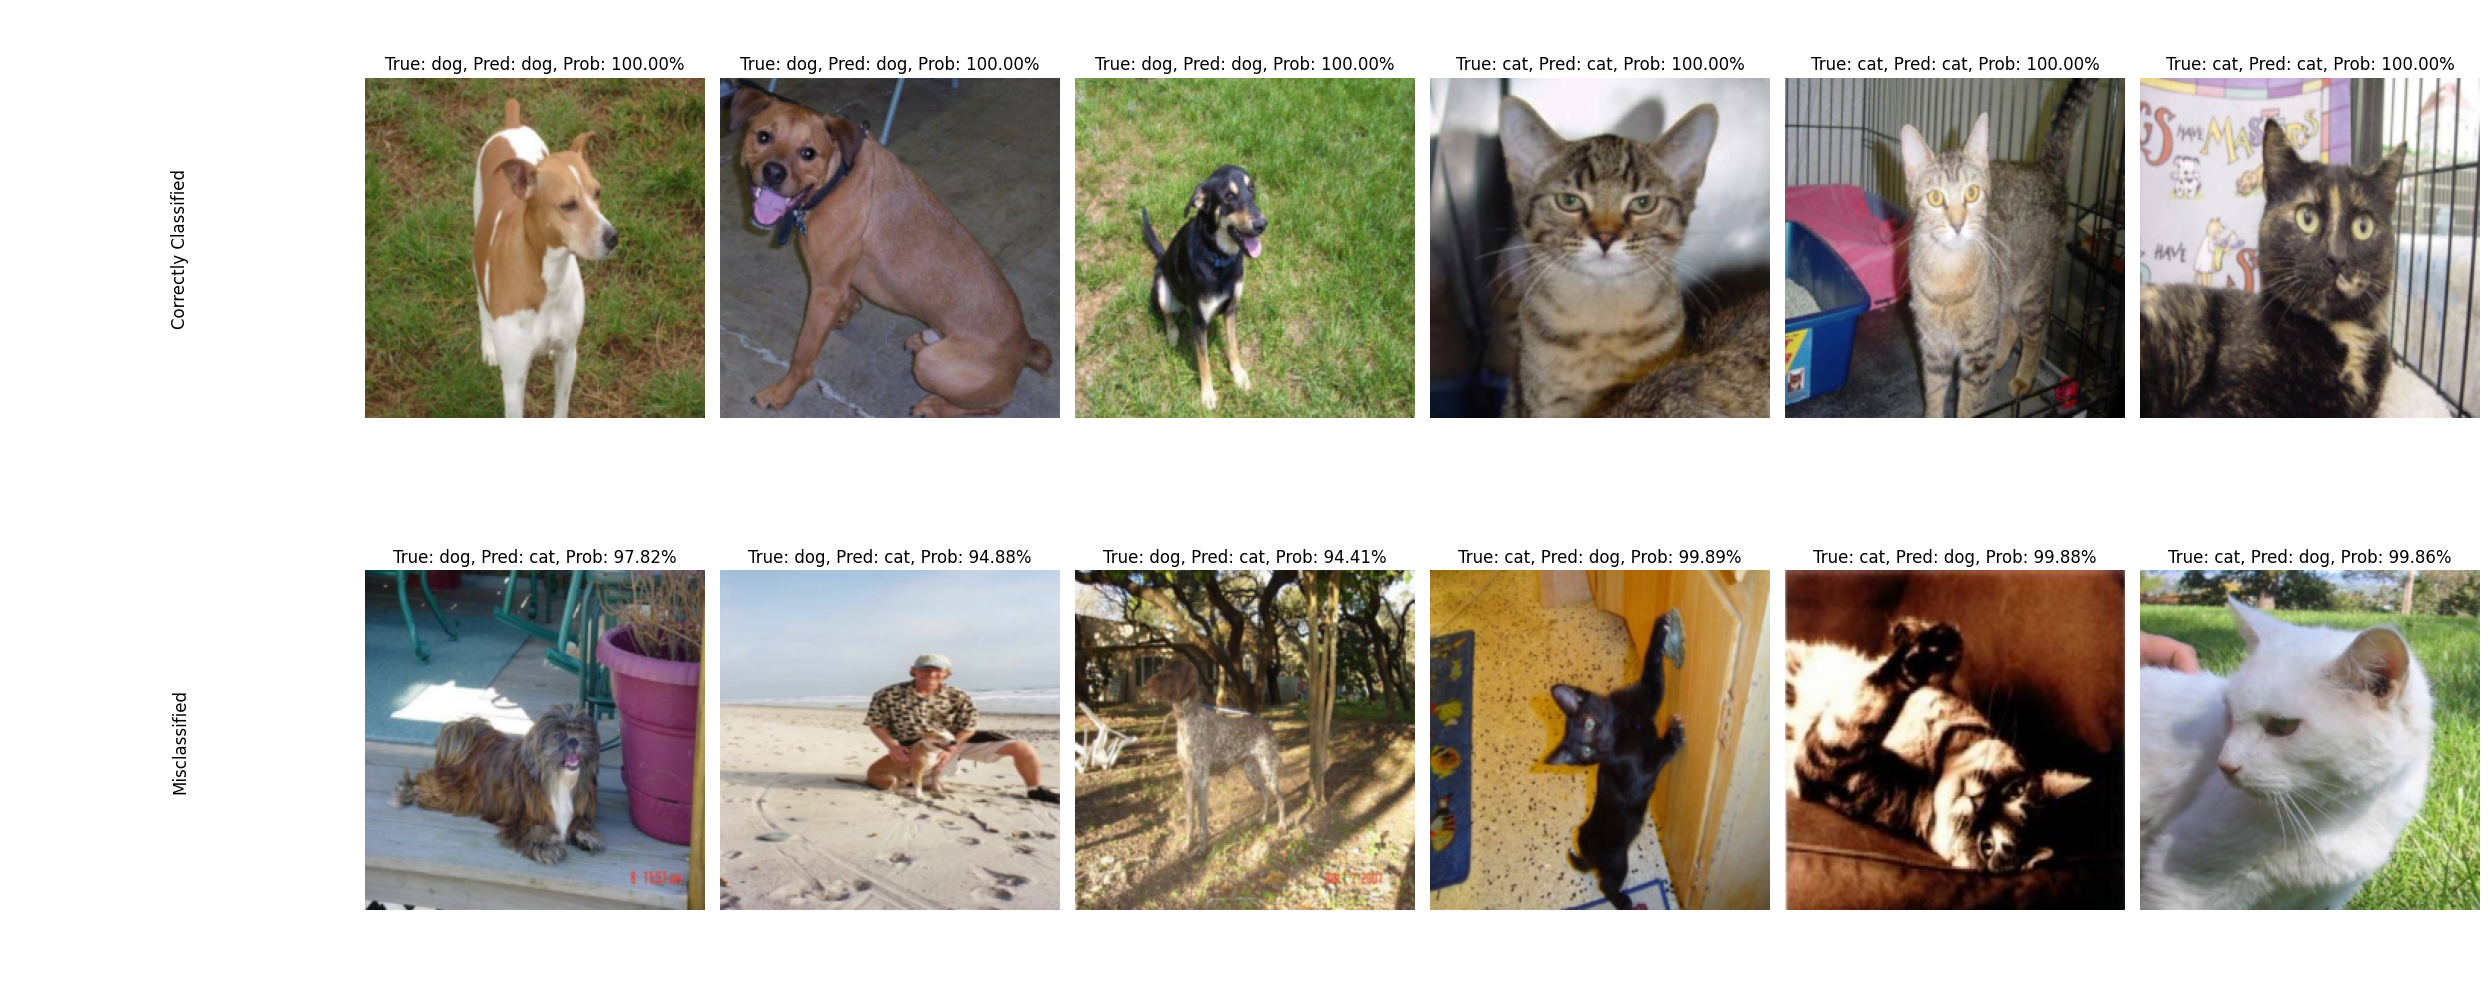
\includegraphics[width=1\textwidth]{figures/predict_images.png}
    \caption{Misclassified and correctly classified images.}
    \label{fig:prediction}
    \vspace*{-0.7cm}
\end{figure}

From the misclassified images, we see that may some more data augmentation could be applied to improve the model's performance.
For example, the cat that rotate its head by almost 90 degrees. Moreover, the model may be improved by adding more crop-scale augmentation.